% Foliensatz: "AFu-Kurs nach DJ4UF" von DK0TU, Amateurfunkgruppe der TU Berlin
% Lizenz: CC BY-NC-SA 3.0 de (http://creativecommons.org/licenses/by-nc-sa/3.0/de/)
% Autoren: Sebastian Lange <dl7bst@dk0tu.de>
% Korrekturen: Lars Weiler <dc4lw@darc.de>

\documentclass[aspectratio=169]{beamer}

\usepackage[ngerman]{babel} % deutsche Worttrennung etc.
\usepackage[utf8]{inputenc} % UTF8 Text

\usepackage[super, comma, numbers, square, sort]{natbib}

\usepackage{hyperref}       % Hyperref Package für bessere Referenzen (todo)
\hypersetup{
	colorlinks=false,       %   false: boxed links; true: colored links
    %linkcolor=white,       %   color of internal links (change box color with linkbordercolor)
    citecolor=red,          %   color of links to bibliography
    filecolor=white,        %   color of file links
    urlcolor=blue           %   color of external links
}

\usepackage{multirow}
\usepackage{wasysym}  % Math Symbols like \permil
%\usepackage{colortbl}
%\usepackage{subscript}
%\usepackage{caption}
%\usepackage{setspace}
%\usepackage{xcolor}        % benutze CodeListe

% Footnote
%\usepackage{hanging}
%
%\setbeamertemplate{footnote}{%
%  \hangpara{2em}{1}%
%  \makebox[2em][l]{\insertfootnotemark}\footnotesize\insertfootnotetext\par%
%}


%\usepackage{pgf}
%\usepackage{tikz}
%\usetikzlibrary{arrows,automata}
%\usetikzlibrary{positioning}
%
%\tikzset{
%    state/.style={
%           rectangle,
%           rounded corners,
%           draw=black, very thick,
%           minimum height=2em,
%           minimum width=2pt,
%           inner sep=2pt,
%           text centered,
%           },
%}

%\usepackage{listings}
%\lstset{basicstyle=\small, numberstyle=\tiny, extendedchars=true, numbers=left, numbersep=5pt}
%\lstset{showtabs=false, showspaces=false, showstringspaces=false}
%%\lstset{backgroundcolor=\color{white!75!lightgray}, , frame=single}
%%\lstset{backgroundcolor=\color{white}}
%%\lstset{backgroundcolor=none}
%\lstset{keywordstyle=\color{blue!50!gray},  identifierstyle=\color{black}}
%\lstset{commentstyle=\color{green!50!gray}, stringstyle=\color{red!50!gray}}
%\lstset{language=C, fontadjust=true, tabsize=2, breaklines=true}
%\lstset{backgroundcolor=\color{white!75!lightgray}, caption=\lstname, frame=single}
%\lstset{emphstyle=\color{black}\fbox}
%
%% Keine "Listing:"-Caption
%\captionsetup{labelformat=empty,labelsep=none}
%
%% für mathematische Umgebungen
%\usepackage{amsmath,amsfonts,amssymb}
%
%\lstdefinestyle{Bash}{
%language=Bash,
%frame=single,
%rulecolor=\color{black},
%backgroundcolor=\color{gray!50},
%keywordstyle=\color{black},
%identifierstyle=,
%commentstyle=\color{black},
%stringstyle=\color{magenta!65!white},
%showstringspaces=false,
%basicstyle=\footnotesize\ttfamily\color{black},
%numbers=none,
%breaklines=true,
%captionpos=b
%}

%\usepackage{listings}
%
%\lstdefinestyle{basic}{
%    captionpos=t,%
%    basicstyle=\footnotesize\ttfamily,%
%    numberstyle=\tiny,%
%    numbers=left,%
%    stepnumber=1,%
%    frame=single,%
%    showspaces=false,%
%    showstringspaces=false,%
%    showtabs=false,%
%    %
%    keywordstyle=\color{blue},%
%    identifierstyle=,%
%    commentstyle=\color{gray},%
%    stringstyle=\color{magenta}%
%}



% fließende Boxen haben keinen Abstand
%\fboxsep0mm

% inkludiere Creative Commons Helper
%%%%%%%%%%%%%%%%%%%%%%%%%%%%%%%%%%%%%%%%%%%%%%%%%%%%%%%%%%%%%%%%
%% ccBeamer 0.1, 2007-07-02                                   %%
%% Written by Sebastian Pipping <webmaster@hartwork.org>      %%
%% ---------------------------------------------------------- %%
%% Licensed under Creative Commons Attribution-ShareAlike 3.0 %%
%% http://creativecommons.org/licenses/by-sa/3.0/             %%
%%%%%%%%%%%%%%%%%%%%%%%%%%%%%%%%%%%%%%%%%%%%%%%%%%%%%%%%%%%%%%%%


%% Images
\newcommand{\CcImageBy}[1]{%
	
\includegraphics[scale=#1]{texdata/creative_commons/cc_by_30.pdf}%
}
\newcommand{\CcImageCc}[1]{%
	
\includegraphics[scale=#1]{texdata/creative_commons/cc_cc_30.pdf}%
}
\newcommand{\CcImageDevNations}[1]{%
	
\includegraphics[scale=#1]{texdata/creative_commons/cc_dev_nations_30.pdf}%
}
\newcommand{\CcImageNc}[1]{%
	
\includegraphics[scale=#1]{texdata/creative_commons/cc_nc_30.pdf}%
}
\newcommand{\CcImageNd}[1]{%
	
\includegraphics[scale=#1]{texdata/creative_commons/cc_nd_30.pdf}%
}
\newcommand{\CcImagePd}[1]{%
	
\includegraphics[scale=#1]{texdata/creative_commons/cc_pd_30.pdf}%
}
\newcommand{\CcImageSa}[1]{%
	
\includegraphics[scale=#1]{texdata/creative_commons/cc_sa_30.pdf}%
}
\newcommand{\CcImageSampling}[1]{%
	
\includegraphics[scale=#1]{texdata/creative_commons/cc_sampling_30.pdf}%
}
\newcommand{\CcImageSamplingPlus}[1]{%
	
\includegraphics[scale=#1]{texdata/creative_commons/cc_sampling_plus_30.pdf}%
}


%% Groups
\newcommand{\CcGroupBy}[2]{% zoom, gap
	\CcImageCc{#1}\hspace*{#2}\CcImageBy{#1}%
}
\newcommand{\CcGroupByNc}[2]{% zoom, gap
	\CcImageCc{#1}\hspace*{#2}\CcImageBy{#1}\hspace*{#2}\CcImageNc{#1}%
}
\newcommand{\CcGroupByNcNd}[2]{% zoom, gap
	\CcImageCc{#1}\hspace*{#2}\CcImageBy{#1}\hspace*{#2}\CcImageNc{#1}\hspace*{#2}\CcImageNd{#1}%
}
\newcommand{\CcGroupByNcSa}[2]{% zoom, gap
	\CcImageCc{#1}\hspace*{#2}\CcImageBy{#1}\hspace*{#2}\CcImageNc{#1}\hspace*{#2}\CcImageSa{#1}%
}
\newcommand{\CcGroupByNd}[2]{% zoom, gap
	\CcImageCc{#1}\hspace*{#2}\CcImageBy{#1}\hspace*{#2}\CcImageNd{#1}%
}
\newcommand{\CcGroupBySa}[2]{% zoom, gap
	\CcImageCc{#1}\hspace*{#2}\CcImageBy{#1}\hspace*{#2}\CcImageSa{#1}%
}
\newcommand{\CcGroupDevNations}[2]{% zoom, gap
	\CcImageCc{#1}\hspace*{#2}\CcImageDevNations{#1}%
}
\newcommand{\CcGroupNcSampling}[2]{% zoom, gap
	\CcImageCc{#1}\hspace*{#2}\CcImageNc{#1}\hspace*{#2}\CcImageSampling{#1}%
}
\newcommand{\CcGroupPd}[1]{% zoom
	\CcImagePd{#1}%
}
\newcommand{\CcGroupSampling}[1]{% zoom
	\CcImageSampling{#1}%
}
\newcommand{\CcGroupSamplingPlus}[1]{% zoom
	\CcImageSamplingPlus{#1}%
}


%% Text
\newcommand{\CcLongnameBy}{Attribution}
\newcommand{\CcLongnameByNc}{Attribution-NonCommercial}
\newcommand{\CcLongnameByNcNd}{Attribution-NoDerivs}
\newcommand{\CcLongnameByNcSa}{Attribution-NonCommercial-ShareAlike}
\newcommand{\CcLongnameByNd}{Attribution-NoDerivs}
\newcommand{\CcLongnameBySa}{Attribution-ShareAlike}

\newcommand{\CcNote}[1]{% longname
	This work is licensed under the \textit{Creative Commons #1 3.0 License}.%
}


% generelles Thema auswählen
\usetheme{Goettingen} %Berlin spart ohne Sidebar allerdings angenehm Platz
% AnnArbor | Antibes | Bergen | Berkeley | Berlin | Boadilla | boxes | CambridgeUS | Copenhagen | Darmstadt | default | Dresden | Frankfurt | Goettingen | Hannover | Ilmenau | JuanLesPins | Luebeck | Madrid | Malmoe | Marburg | Montpellier | PaloAlto | Pittsburgh | Rochester | Singapore | Szeged | Warsaw

% Farben wählen
\usecolortheme{beetle}
% beaver | beetle | crane | default | dolphin | dove | fly | lily | orchid | rose | seagull | seahorse | sidebartab | structure | whale | wolverine

% Setze alle Farben auf Grau und Weiß
%\definecolor{craneorange}{RGB}{64,64,64}
%\definecolor{craneblue}{RGB}{255,255,255}

% Schriftart wählen
\usefonttheme{default}
% default | professionalfonts | serif | structurebold | structureitalicserif | structuresmallcapsserif

% Innere Themen(Kopf-, Fuß-, Sidebar usw)
%\useinnertheme{default}
\useinnertheme{circles}
% default | inmargin | rectangles | rounded | circles

% Äußere Themen (Anordnung der inneren, grenzen der Folien etc.)
\useoutertheme{infolines}
% default | infolines | miniframes | shadow | sidebar | smoothbars | smoothtree | split | tree

% Deaktiviere Navigations-Symbole ({} -> leer)
\setbeamertemplate{navigation symbols}{}
%\setbeamertemplate{navigation symbols}{\large \ifnum \insertframenumber <10 0\fi\insertframenumber/\inserttotalframenumber\vspace*{0.2ex}}

% Zeige ein Hintergrundbild
\setbeamertemplate{background canvas}{
        \hspace*{-2.0cm}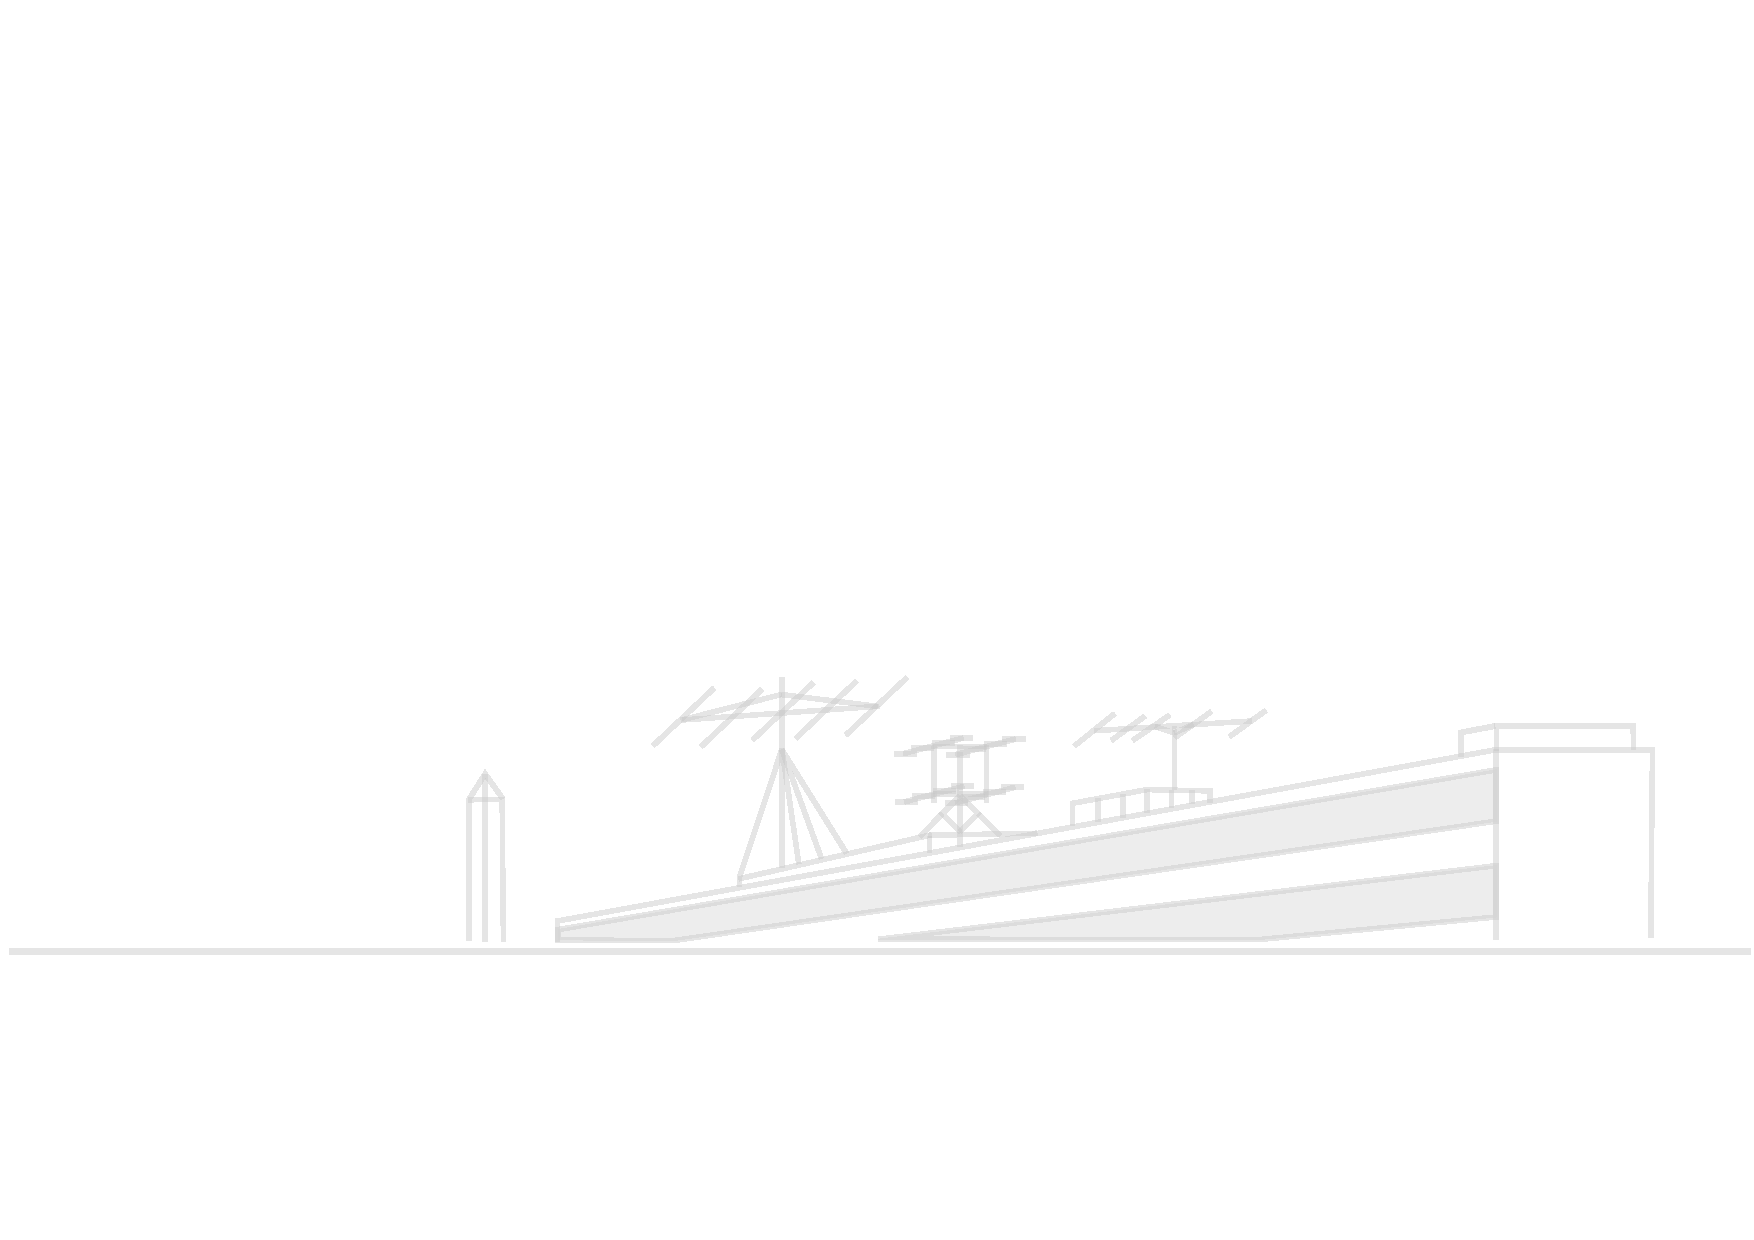
\includegraphics[width=17.8cm]{texdata/dk0tu_rooftop_background.pdf}
}

% Foliennummer einfügen
\setbeamertemplate{footline}[frame number]
%\setbeamertemplate{footline}{}

% Ändere das Zeichen vor jedem item
%\setbeamertemplate{itemize item}{\color{craneorange}$\blacktriangleright$}
%\setbeamertemplate{itemize subitem}{\color{craneorange}$\triangleright$}
%\setbeamertemplate{itemize subsubitem}{\color{craneorange}$\blacktriangleright$}

% Ändert die Blöcke 
\setbeamertemplate{blocks}[rounded][shadow=true]
% default | rounded [shadow=true|false]

%
% Eigene Kommandos
%

% Hack to get natbib and beamer working together. "The beamer user guide suggests
% that only the manual bibliography entry approach is supported"
% on some system it works out of the box, sometimes you need the hack :-(
% so check it --dl7bst
\ifdefined\newblock
    \relax
\else
    \newcommand{\newblock}{}
\fi

% \includedia command to generate png out of a dia file
% NEEDS installed dia and pdflatex option --shell-escape
\newcommand{\includedia}[1]{
    \immediate\write18{/usr/bin/dia #1.dia -e #1_diatmp.png -t png}
}

% RICHIG GROSSER FONT!
\newfont{\bigfont}{cmr10 at 144pt}
\newfont{\smallfont}{cmr10 at 8pt}

% Römische Ziffern
\makeatletter
\newcommand{\rmnum}[1]{\romannumeral #1}
\newcommand{\Rmnum}[1]{\expandafter\@slowromancap\romannumeral #1@}
\makeatother

% Schwarze Überschrift
%\setbeamercolor{frametitle}{fg=black}
%\setbeamercolor{title}{fg=black}

% Item- und Box-Farben
\definecolor{deepBlue}{HTML}{000066}
\setbeamercolor{itemize item}{fg=deepBlue}
\setbeamercolor{itemize subitem}{fg=deepBlue}
\setbeamercolor{description item}{fg=deepBlue}
\setbeamercolor{block title}{fg=deepBlue!100, bg=blue!15}
\setbeamercolor{block body}{fg=black, bg=blue!5}
\setbeamercolor{block title alerted}{fg=deepBlue, bg=red!75}
\setbeamercolor{block body alerted}{fg=black, bg=red!15}
\setbeamercolor*{block title example}{fg=blue!50, bg=blue!10}
\setbeamercolor*{block body example}{fg= blue, bg=blue!5}

%\setbeamercolor{section in head/foot}{parent=palette primary}
%\setbeamercolor{subsection in head/foot}{parent=palette secondary}
%\setbeamercolor{sidebar}{fg=darkblue,bg=yellow!90!orange}
%\setbeamercolor{title in sidebar}{fg=darkblue}
%\setbeamercolor{author in sidebar}{fg=darkblue}
%\setbeamercolor{section in sidebar}{fg=darkblue!10!black}
%\setbeamercolor{subsection in sidebar}{fg=darkblue!50!black}

% Titlepage Infos
\title{AFu-Kurs nach DJ4UF}
\author[DKØTU]{DKØTU\\ \footnotesize{Amateurfunkgruppe der TU Berlin}}
\institute[DKØTU]{\url{http://www.dk0tu.de} }

% PDF-Eigenschaften
\subject{DK0TU-Amateurfunkkurs nach DJ4UF}
\keywords{Amateurfunk Kurs HAM Radio Course CC-BY-NC-SA OpenSource TU Berlin DK0TU}

\subtitle{Betriebstechnik/Vorschriften 08: \\
  Amateurfunkstellen \\[2em]}
\date{Stand 07.11.2017}
 \begin{document}

\begin{frame}
    \titlepage
    \vfill
    \begin{center}
        \ccbyncsaeu\\
        {\tiny This work is licensed under the \em{Creative Commons Attribution-NonCommercial-ShareAlike 3.0 License}.}\\[0.5ex]
         \tiny Amateurfunkgruppe der Technische Universität Berlin (AfuTUB), DKØTU
         %\includegraphics[scale=0.5]{img/DK0TU_Logo.pdf}
    \end{center}
\end{frame}


\section[]{Einleitung}

\begin{frame}

    \frametitle{Personengebundene Rufzeichen}

    {\Large Personengebundene Rufzeichen}\\[1.5em]

    \begin{itemize}
        \item Das normale Feld-, Wald- und Wiesenrufzeichen.
        \item Darf nur vom Rufzeicheninhaber persönlich benutzt werden\\
          (eben \emph{personengebunden}).
        \item Gibts in den beiden Geschmacksrichtungen ``Klasse A'' und ``Klasse E''.
    \end{itemize}

    \begin{center}
        \Large{\textbf{Und was gibt es noch?}}\\(Darum geht es hier.)\\[1em]
    \end{center}
    
    \begin{itemize}
        \item Rufzeichen für verschiedene Sorten \textbf{Amateurfunkstellen}
        \item Rufzeichen für Ausbildungsfunkbetrieb
    \end{itemize}

\end{frame}

\section[]{Formales}

\begin{frame}
  \frametitle{Einleitung: Amateurfunkstellen}

  Erst einmal klären:

  \begin{center}
    \Large{Was ist eine Amateurfunkstelle?}
  \end{center}

\end{frame}

\begin{frame}
  \frametitle{Definition Amateurfunkstelle}

  Laut \textbf{Radio Regulations} (RR = VO Funk) und \textbf{AFuG}:

  \begin{center}
    ``Eine Amateurfunkstelle ist eine Funkstelle des Amateurfunkdienstes.''\\[1em]
  \end{center}

  Hintergrund: \\
  Es gibt viele verschiedene Funkdienste. Der Amateurfunkdienst ist einer davon.\\[2em]

  \uncover<2>{
      Ok\ldots\ -- und was ist eine \textbf{Funkstelle}?
  }

\end{frame}

\begin{frame}
  \frametitle{Definition Funkstelle}

  Mehrere Transceiver im Shack, Stations-PC, Stromversorgung, Kleinkram wie
  Mikrofone und Morsetasten, verschiedene Antennen auf dem Dach: Alles
  zusammen bildet eine ``Funkstelle des Amateurfunkdienstes.''\\[2em]

  Amtliche Definition Funkstelle\\[1em]

  \begin{quote}
    Ein oder mehrere Sender oder Empfänger oder eine Zusammenschaltung von
    Sendern und Empfängern einschließlich der Zusatzeinrichtungen, die zum
    Ausüben eines Funkdienstes an einem Ort erforderlich sind.
  \end{quote}

\end{frame}

\begin{frame}


    {\Large \textbf{Funkdienst-spezifisch!}}\\[1em]

    Auf dem Shacktisch von Funkamteurin Gabi tummeln sich ein
    Kurzwellentransceiver, ein VHF/UHF-Duobander und ihr Smartphone.\\[1em]

    Wie viele Funkstellen?\\[1em]

  \uncover<2>{
    Das ergibt zwei Funkstellen.
  }
\end{frame}

\section{Funken im Team}

\subsection{Clubstationen}

\begin{frame}
  \frametitle{Clubstationsrufzeichen}

  \begin{center}
    \Large Clubstationsrufzeichen
  \end{center}

  \begin{itemize}[<+->]
    \item Ziel: Funken als Team unter einheitlichem Rufzeichen.
    \item Beispiel: Contestteilnahme, Fieldday.
    \item Beispiel: DARC-Sonder-DOK vergeben (das darf nur eine Clubstation).
    \item Erlaubt: Wechselnde Operator (alle mit eigener Zulassung).
    \item Klasse A: Nur wenn Op und Clubstationsrufzeichen \emph{beide} Klasse A.
    \item Erlaubt: Wechselnde Standorte.
    \item In der Praxis egal: Welche oder wessen Station dabei tatsächlich benutzt wird.
    \item Erlaubt: Große Funkstelle, mehrere Sender, mehrere Ops \emph{am selben Standort.}
    \item Nicht erlaubt ohne spezielle Genehmigung der BNetzA:\\
          \emph{Gleichzeitige} Aktivierung mehrerer Standorte.
    \item Ein an der Clubstation funkender Funkamateur \emph{muss} ihr Rufzeichen benutzen.
  \end{itemize}

\end{frame}

\begin{frame}
  \frametitle{Clubstationsrufzeichen}

  Klasse A: \textbf{DAØ, DA3, DFØ, DKØ, DLØ, DP3--9, DQ, DR}\\ 
  Klasse A mit nur einstelligem Suffix: \textbf{DA3, DP3--9, DQ, DR}\\ 
  Klasse A an exterritorialen Standorten: \textbf{DPØ--1}\\[1em]
  Klasse E: \textbf{DNØ}\footnote{18 Rufzeichen vergeben, Stand 10/2016}\\ 
  Klasse E mit nur einstelligem Suffix: \textbf{DA7--9}\\ 
  Klasse E an exterritorialen Standorten: \textbf{DP2} \\[1em]

  Beispiele:

  \begin{itemize}
    \item \textbf{DKØTU} Clubstationsrufzeichen Amateurfunkgruppe der TU Berlin.
    \item \textbf{DAØCCC} Clubstationsrufzeichen des CCC.
    \item \textbf{DLØABT} Clubstationsrufzeichen des DARC-DOK D25.
  \end{itemize}

\end{frame}

\begin{frame}
  \frametitle{Clubstationsrufzeichen}

    Den Antrag auf Zuteilung eines Clubstationsrufzeichens stellt der OVV\footnote{o.ä. ``Leiter einer Gruppe von Funkamateuren''}.\\ 
    Der OVV nennt im Antrag einen Verantwortlichen,\\
    auf den das Rufzeichen zugelassen wird.\\ [1.5em]

  Die Zulassung wird widerrufen

  \begin{itemize}
    \item wenn der Clubstationsverantwortliche kein persönliches Rufzeichen mehr hat,
    \item wenn der OVV den Widerruf beantragt,
    \item wenn der OV\footnote{o.ä. ``Gruppe von Funkamateuren''} aufgelöst wird.\\ [1.5em]
  \end{itemize}

\end{frame}

\begin{frame}
    \frametitle{DXpeditionen}

    \begin{center}
      Deutsche Clubstationsrufzeichen berechtigen nicht zum Funken im
      Ausland\\
      nach CEPT-Empfehlung T/R 61-01.\\[2em]

      Deutsche DXpeditionen im Ausland
      beantragen \textbf{dort} eine \textbf{Gastgenehmigung}!
    \end{center}

\end{frame}

\subsection{Kurzzeit-Sonderstationen}

\begin{frame}
  \frametitle{Kurzzeit-Sonderstationen}

  \textbf{DAØ} -- Kurzzeit-Sonderrufzeichen

  Für besondere Anlässe: Messen, Ausstellungen, Jubiläen, ... \\[3em]

  \uncover<2>{
    Nicht zu verwechseln mit Sonder-DOKs. Die werden für ähnliche Zwecke
    vom DARC ausgegeben, sind nicht amtlich, kosten nichts,
    dürfen aber nur von einer Clubstation aus verteilt werden.
  }


\end{frame}

\section{Baken und Relais}


\begin{frame}
  \frametitle{Baken und Relais}

  \textbf{DBØ} und \textbf{DMØ, DOØ}\footnote{seit 2005 und deshalb nicht
  prüfungsrelevant} -- Relaisfunkstellen (\& Digipeater), Funkbaken \\[1em]

  \uncover<2>{
    Offizielle Bezeichnung:\\
    ``\textbf{fernbediente oder automatisch arbeitende Amateurfunkstelle}'' \\[3em]
  }

\end{frame}

\subsection{Baken}

\begin{frame}
  \frametitle{Funkbaken}

  Laut AFuV:

  \begin{quote}
    Eine ``Funkbake'' ist eine \textbf{automatisch arbeitende} Amateurfunk-Sendeanlage
    (auch in Satelliten), die \textbf{selbsttätig} Aussendungen zur
    Feldstärkebeobachtung oder zu Empfangsversuchen erzeugt.\footnote{
      Weltweite Liste von ca. 700 HF Beacons: \ExternalLink\url{http://dl8wx.de/baken_kw.htm}}\\[1.5em]
  \end{quote}

  \uncover<2>{
    Bakenbetrieb, \emph{während man anwesend ist,} darf jeder --
    das ergibt keine Funkbake in diesem Sinne (man recherchiere ``WSPR'').\\[1em]
    Für eine \textbf{automatisch arbeitende} Funkbake braucht man dagegen ein eigenes,
    von der BNetzA ausgestelltes Rufzeichen.
  }

\end{frame}

\begin{frame}
  \frametitle{Auflagen für Funkbaken}

  Rufzeichen für automatisch arbeitende Amateurfunk-Sendeanlagen\\
  sind verbunden mit Auflagen:\\[1em]

  \begin{itemize}
    \item Zuweisung einer festen Frequenz durch die BNetzA.
    \item Betrieb wird für einen festen Standort genehmigt,
    \item mit festgelegter maximaler Sendeleistung oder EIRP.
  \end{itemize}

\end{frame}

\begin{frame}
  \frametitle{Funkbaken: IARU Bakensystem}

  \begin{center}
    \Large International Beacon Project der IARU
  \end{center}

  Globales HF Bakensystem \textbf{IBP} mit 18 Baken verteilt über die
  ganze Erde.

  \begin{itemize}[<+->]
    \item QRGs 14100, 18110, 21150, 24930 und 28200 kHz, also Kurzwelle ab 20~m.
    \item Senden in CW: Call, dann 4x Träger, je 1x mit 100, 10, 1 und 0,1 Watt.
    \item Nach genau 10 Sekunden ist die nächste Bake (woanders) dran.
    \item Fester Fahrplan -- man braucht nicht morsen können, um zu wissen, was man gerade hört,
          sondern nur eine sekundengenaue Uhr.  (Siehe auch\footnote{\ExternalLink\url{http://www.dl1dlf.de/beacons.php}}.)
    \item Alle 3 Minuten wiederholt sich das ganze Programm.
    \item Alle 18 Baken senden auf allen fünf Frequenzen.
  \end{itemize}

  \begin{center}
    Link zu einem Hörbeispiel: \texttt{4U1UN} \hyperlink{refs}{\cite{ibp}}
  \end{center}
\end{frame}


\begin{frame}
  \frametitle{Funkbaken: IARU Bakensystem\hyperlink{refs}{\cite{ibp}} (tabellarisch)}

  \begin{center}
    \scriptsize

    {Bakenfahrplan -- alle drei Minuten wiederholt sich das}
    
    \begin{tabular}{|l|l|l|l|l|l|l|}\hline
      Call   & Location                          & 14100 & 18110 & 21150 & 24930 & 28200 \\ \hline \hline
      4U1UN  & United Nations                    & 00:00 & 00:10 & 00:20 & 00:30 & 00:40 \\ \hline
      VE8AT  & Canada                            & 00:10 & 00:20 & 00:30 & 00:40 & 00:50 \\ \hline
      W6WX   & United States                     & 00:20 & 00:30 & 00:40 & 00:50 & 01:00 \\ \hline
      KH6WO  & Hawaii                            & 00:30 & 00:40 & 00:50 & 01:00 & 01:10 \\ \hline
      ZL6B   & New Zealand                       & 00:40 & 00:50 & 01:00 & 01:10 & 01:20 \\ \hline
      VK6RBP & Australia                         & 00:50 & 01:00 & 01:10 & 01:20 & 01:30 \\ \hline
      JA2IGY & Japan                             & 01:00 & 01:10 & 01:20 & 01:30 & 01:40 \\ \hline
      RR9O   & Russia                            & 01:10 & 01:20 & 01:30 & 01:40 & 01:50 \\ \hline
      VR2B   & Hong Kong                         & 01:20 & 01:30 & 01:40 & 01:50 & 02:00 \\ \hline
      4S7B   & Sri Lanka                         & 01:30 & 01:40 & 01:50 & 02:00 & 02:10 \\ \hline
      ZS6DN  & South Africa                      & 01:40 & 01:50 & 02:00 & 02:10 & 02:20 \\ \hline
      5Z4B   & Kenya                             & 01:50 & 02:00 & 02:10 & 02:20 & 02:30 \\ \hline
      4X6TU  & Israel                            & 02:00 & 02:10 & 02:20 & 02:30 & 02:40 \\ \hline
      OH2B   & Finland                           & 02:10 & 02:20 & 02:30 & 02:40 & 02:50 \\ \hline
      CS3B   & Madeira                           & 02:20 & 02:30 & 02:40 & 02:50 & 00:00 \\ \hline
      LU4AA  & Argentina                         & 02:30 & 02:40 & 02:50 & 00:00 & 00:10 \\ \hline
      OA4B   & Peru                              & 02:40 & 02:50 & 00:00 & 00:10 & 00:20 \\ \hline
      YV5B   & Venezuela                         & 02:50 & 00:00 & 00:10 & 00:20 & 00:30 \\ \hline
    \end{tabular}
  \end{center}

\end{frame}


\begin{frame}
  \frametitle{Funkbaken: IARU Baken QRGs}

  \begin{center}
    \Large Auf den Baken-QRGs kein sonstiger Sendebetrieb!\footnote{Mehr dann in \texttt{BV09} (Betriebsarten, Sendearten, Frequenzen)}
  \end{center}

  Beispiele:
    
  \begin{itemize}

    \item Für IBP freizuhalten:\\
    14099-14101, 18109-18111, 21149-21151, 24929-24931, 28190-28225 kHz

    \item VHF: 144,400 - 144,490 MHz
    
    \item UHF: 432,800 - 432,990 MHz
  \end{itemize}
\end{frame}

\begin{frame}
  \frametitle{Fuchsjagd}

  {\Large Fuchsjagd}\\[1.5em]

  Fuchsjagdsender sind Kleinsender, Leistung weniger als 5 Watt, die
  im Gelände verteilt sind.  Eine ``Fuchsjagd'' ist ein
  funksportlicher Wettbewerb, bei denen Fuchsjagdsender durch Peilung
  mit passenden Peilempfängern zu finden sind.  Benutzt werden
  üblicherweise die Bänder 80~m, 2~m und 70~cm.\\[1.5em]

  Fuchsjagdsender dürfen durch lizensierte Funkamateure ohne weitere
  Genehmigung ausgelegt und betrieben werden.\\[1.5em]

  Die Fuchsjagdteilnehmer brauchen ohnehin keine Lizenz, da sie nur empfangen.

\end{frame}

\begin{frame}

\frametitle{Fuchsjagdkennung}

  Die Fuchjagdsender sind (die einzigen) Funkstellen des
  Amateurfunkdienstes, \textbf{die keine Rufzeichen auszusenden
  brauchen,} sondern nur Peilkennungen in CW.  Als Peilkennungen sind
  erlaubt: MO, MOE, MOI, MOS, MOH und MO5\footnote{Nochmal: Das sind
  keine Rufzeichen! M wäre Großbritannien.}.\\[1.5em]

  Diese CW-Kennungen, 1972 festgelegt, waren damals auch ohne
  Microcontroller technisch darstellbar.

\end{frame}

\subsection{Relaisfunkstellen}

\begin{frame}
   \frametitle{Relaisfunkstelle -- Beispiel}

   Das \textbf{Spandau-Relais DBØSP} auf einem exponierten Standort
   (Fernmeldeturm Schäferberg) empfängt auf 145.000~MHz und sendet,
   was es dort hört, auf 145.600~MHz wieder aus.\footnote{Außerdem QRV auf
   70cm und Echolink, siehe \url{http://db0sp.darc.de/technik.html}}\\[1.5em]

   DBØSP deckt Berlin bestens ab.  Ich\footnote{DJ3EI} habe schon im
   Wald südlich von Grünau mit simpler Handfunke problemlos quer durch
   ganz Berlin ``über das Relais'' gearbeitet.
\end{frame}

\begin{frame}
   \frametitle{Relais -- schrecklich und schön!}

   Auf Relais finden sich gelegentlich schräge Vögel -- und leider ab
   und zu destruktive Störer.  Dann gilt: \textbf{``Don't feed the
   troll!''} Man reagiere möglichst wenig und vermeide es, dem Störer
   Empfangsbestätigungen oder Erfolgsmeldungen zu geben.\\[1em]

   Relaisfunk muss man nicht mögen, kann es aber. Es kann sehr nett
   sein, z.B. in der Mittagspause oder beim Pendeln über ein Relais zu
   arbeiten!\\[1em]

   Über Relaisverbindungen werden nicht wenige Freundschaften
   geschlossen und gepflegt.

\end{frame}


\begin{frame}
  \frametitle{Relaisfunkstellen (\& Digipeater)}

  \begin{center}
    \Large Relaisfunkstellen
  \end{center}

  Text AFuV: \\[1em]

  \begin{quote}
    Eine ``Relaisfunkstelle'' ist eine \textbf{fernbediente} Amateurfunkstelle
    (auch in Satelliten), die empfangene Amateurfunkaussendungen, Teile davon
    oder sonstige eingespeiste oder eingespeicherte Signale fern ausgelöst
    aussendet und dabei zur Erhöhung der Erreichbarkeit von Amateurfunkstellen
    dient.
  \end{quote}

  \uncover<2>{
      Solange ich anwesend bleibe, kann ich meine Amateurfunkstelle
      durch andere fernsteuern lassen ohne besonderes Rufzeichen
      (zum Beispiel bei APRS üblich).
  }

\end{frame}

\begin{frame}
  \frametitle{Regeln Relaisfunkstellen (\& Digipeater)}

  \begin{itemize}[<+->]
    \item Für fernbediente Station notwendig: \textbf{Rufzeichenzuteilung},
    \item gibts nur für Funkamateure mit Zulassung.
    \item Relaisbetreiber stellt die jederzeitige \textbf{Abschaltbarkeit} sicher.
    \item Betrieb nur auf der ausgewiesenenen \textbf{QRG} der Zuteilung.
    \item Betrieb nur am ausgewiesenenen \textbf{Standort} der Zuteilung.
    \item Betrieb nur mit der maximalen \textbf{Leistung} der Zuteilung.
    \item Max. zulässige Strahlungsleistung $>30$~MHz \textbf{15~Watt
      ERP}\footnote{ERP = Effective radiated power, kommt in \texttt{E18}.}.
    \item Für Frage VD511: Lang andauernder Funkverkehr über ein Relais
      ist \emph{keine} Störung\footnote{im Sinne des § 13 Abs. 4 AFuV}.
    \item Für Frage VA204: Zwischen 27120 und 27410 kHz gibt es kein
      Amateurfunkband (sondern CB-Funk) und also auch kein Afu-Relais.
  \end{itemize}

\end{frame}

\section{Ausbildungsfunk}

\begin{frame}
  \frametitle{Ausbildungsrufzeichen}

  {\Large Ausbildungsfunk}

  \textbf{DN1--DN6}: Ausbildungsrufzeichen Klasse A, \textbf{DN7--DN8}: Klasse E

  \begin{itemize}[<+->]
    \item Funken mit Ausbildungsrufzeichen ohne eigene Lizenz des Funkenden
    \item aber unter \textbf{unmittelbarer Anleitung durch den Ausbilder}.
    \item Zweck: Praktische Prüfungsvorbereitung, \textbf{nicht} blosses Vorführen.
    \item Ausbildungsrufzeichen wird von \textbf{Auszubildenden} benutzt, nie vom Ausbilder,
    \item trotzdem \textbf{personengebunden} an die Person des Ausbilders,
    \item wird von der BNetzA kostenpflichtig unbefristet erteilt.
    \item Pflicht \textbf{Logbuch}führung durch die Auszubildenden,
    \item Logbuch vom Ausbilder zu bestätigen und ein Jahr aufzubewahren.
    \item \textbf{Berechtigungsumfang} (Klasse A oder E) des Ausbilders.
    \item Funken mit deutschem Ausbildungsrufzeichen nicht im Ausland.
    \item Ausbildungsfunkbetrieb hat \textbf{nichts} mit Clubstationsrufzeichen zu tun.
  \end{itemize}

\end{frame}

\section{Besonderes}

\subsection{Besondere Studien}

\begin{frame}
  \frametitle{Besondere Studien}

  {\Large Besondere Studien}\\[1.5em]

  \textbf{DA4--5} - Amateurfunkstelle für besondere experimentelle und
  technisch-wissenschaftliche Studien nach §16 Abs. 2 der AFuV.\\[2em]

  Wenn es sonst nicht erlaubt wäre, kann es eine Sondergenehmigung geben.\\[1em]

  \uncover<2>{
    Zum Beispiel handverlesene Sondergenehmigungen als
    Test, wenn die BNetzA überlegt, ein neues Band für den
    Amateurfunk frei zu geben.
  }

\end{frame}

\subsection{Exterritorial}

\begin{frame}
  \frametitle{Exterritorial}

  {\Large Exterritorial}

  \textbf{DP0--2} - exterritorialen Gebiete, z.B.:

  \begin{itemize}
    \item Polargebiete
    \item Satelliten
    \item Botschaften
  \end{itemize}

  \begin{exampleblock}{Zugewiesene exterritoriale Clubstationen}
    \begin{description}
      \item[DPØISS] Weltraumstation ISS
      \item[DPØGVN] Neumayer-Station Antarktis
      \item[DP1POL] Weitere Antarktis Station
    \end{description}
  \end{exampleblock}

\end{frame}



\section[]{Präfix-Quiz}

\begin{frame}
  \frametitle{Präfix-Quiz}

  \begin{exampleblock}{
    \LARGE
    \begin{center}
      \only<1-2>{DP1, DPØ \\}
      \only<3-4>{DBØ \\}
      \only<5-6>{DO1-9 \\}
      \only<7-8>{DFØ, DKØ, DLØ \\}
      \only<9-10>{DN1-9 \\}
      \only<11-12>{DNØ \\}
      \only<13-14>{DAØ, DQ, DR \\}
      \only<15-16>{DA-DM \\}
      \only<17-18>{DA5U \\}
      \only<19-20>{MO, MOE, MOI, MOS \\}
    \end{center}
    }
    \Large
    \begin{center}
      \only<1,3,5,7,9,11,13,15,17,19>{...? \\}
      \only<2>{Exterritoriale Funkstelle \\}
      \only<4>{Relaisfunkstelle, Digipeater, Funkbake \\}
      \only<6>{Personengebunden Klasse E \\}
      \only<8>{Clubstation Klasse A \\}
      \only<10>{Ausbildungsstation \\}
      \only<12>{Clubstation Klasse E \\}
      \only<14>{Kurzzeitclubstation \\}
      \only<16>{Personengebunden Klasse A \\}
      \only<18>{Experimentelle Sonderstation \\}
      \only<20>{Peilkennungen für Fuchsjagdsender \\}
    \end{center}
  \end{exampleblock}

\end{frame}

\section[]{Zusammen\-fassung}

\begin{frame}
  \frametitle{Zusammenfassung}

  Komplette und korrekte Liste in den aktuellen Amtsblattverfügungen AFu der
  BNetzA\footnote{\ExternalLink\url{http://www.bundesnetzagentur.de/SharedDocs/Downloads/DE/Sachgebiete/Telekommunikation/Unternehmen_Institutionen/Frequenzen/Amateurfunk/AmtsblattverfuegungenAFu/Vfg122005ge228ndertdurcId1833pdf.pdf?__blob=publicationFile&v=4}}\\[2em]

  \dots oder etwas übersichtlicher in der Wikipedia\footnote{\ExternalLink\url{https://de.wikipedia.org/wiki/Amateurfunkrufzeichen}}

\end{frame}

\renewcommand{\refname}{Referenzen}

\begin{frame}
  \frametitle{Referenzen/Links}
  \hypertarget{refs}{}
  \footnotesize

  \begin{thebibliography}{}
    \bibitem{dj4uf} Moltrecht B/V 08: \\
      \url{https://www.darc.de/der-club/referate/ajw/lehrgang-bv/bv08/}
    \bibitem{wp}    Wikipedia DE: \\
      \url{http://de.wikipedia.org/wiki/Amateurfunkrufzeichen} \\
      \url{http://de.wikipedia.org/wiki/Ausbreitungsbake}
    \bibitem{ibp}   NCDXF/IARU Beacon Transmission Schedule: \\
      \url{http://www.ncdxf.org/beacon/beaconschedule.html}
    \bibitem{bpol}  Baken-Politik der IARU Region 1: \\
      \url{http://www.darc.de/referate/hf/baken/}
  \end{thebibliography}

\end{frame}

% Hier könnte noch eine Kontaktfolie stehen

\end{document}

